\section{Capping in E1}

    \margininbox{13.08.09 - Izi, Dan, Jarv}{
Took 27 caps. Used them all. A lot were double or bust, but still around 18 shot holes around 15 centimetres deep, using only a third of the 7.5 Ah SLA battery (24V with the Bosch). Blew a lot of rock. Surveyed out, around 30 m deep.
\mininame{Jarv}}{\logbook}

\subsection{Logbook - 14/08/09}

Back with Gergely -- two more caps some hammer \& chisel action \& we
were through! Placed a rawl (stainless) for pitch.

New chamber is 23 m with 4 m climb into prior discovered stuff.

Rubble on floor -- dug for $\approx$ 10'.

Got to bedrock.

No better nor worst than capped pitch, but not the stunning lead we were hoping for.

\name{Jarvist Frost}



\begin{pagefigure}
      \checkoddpage \ifoddpage \forcerectofloat \else \forceversofloat \fi
    \centering
    \begin{subfigure}{0.49\textwidth}
        \frame{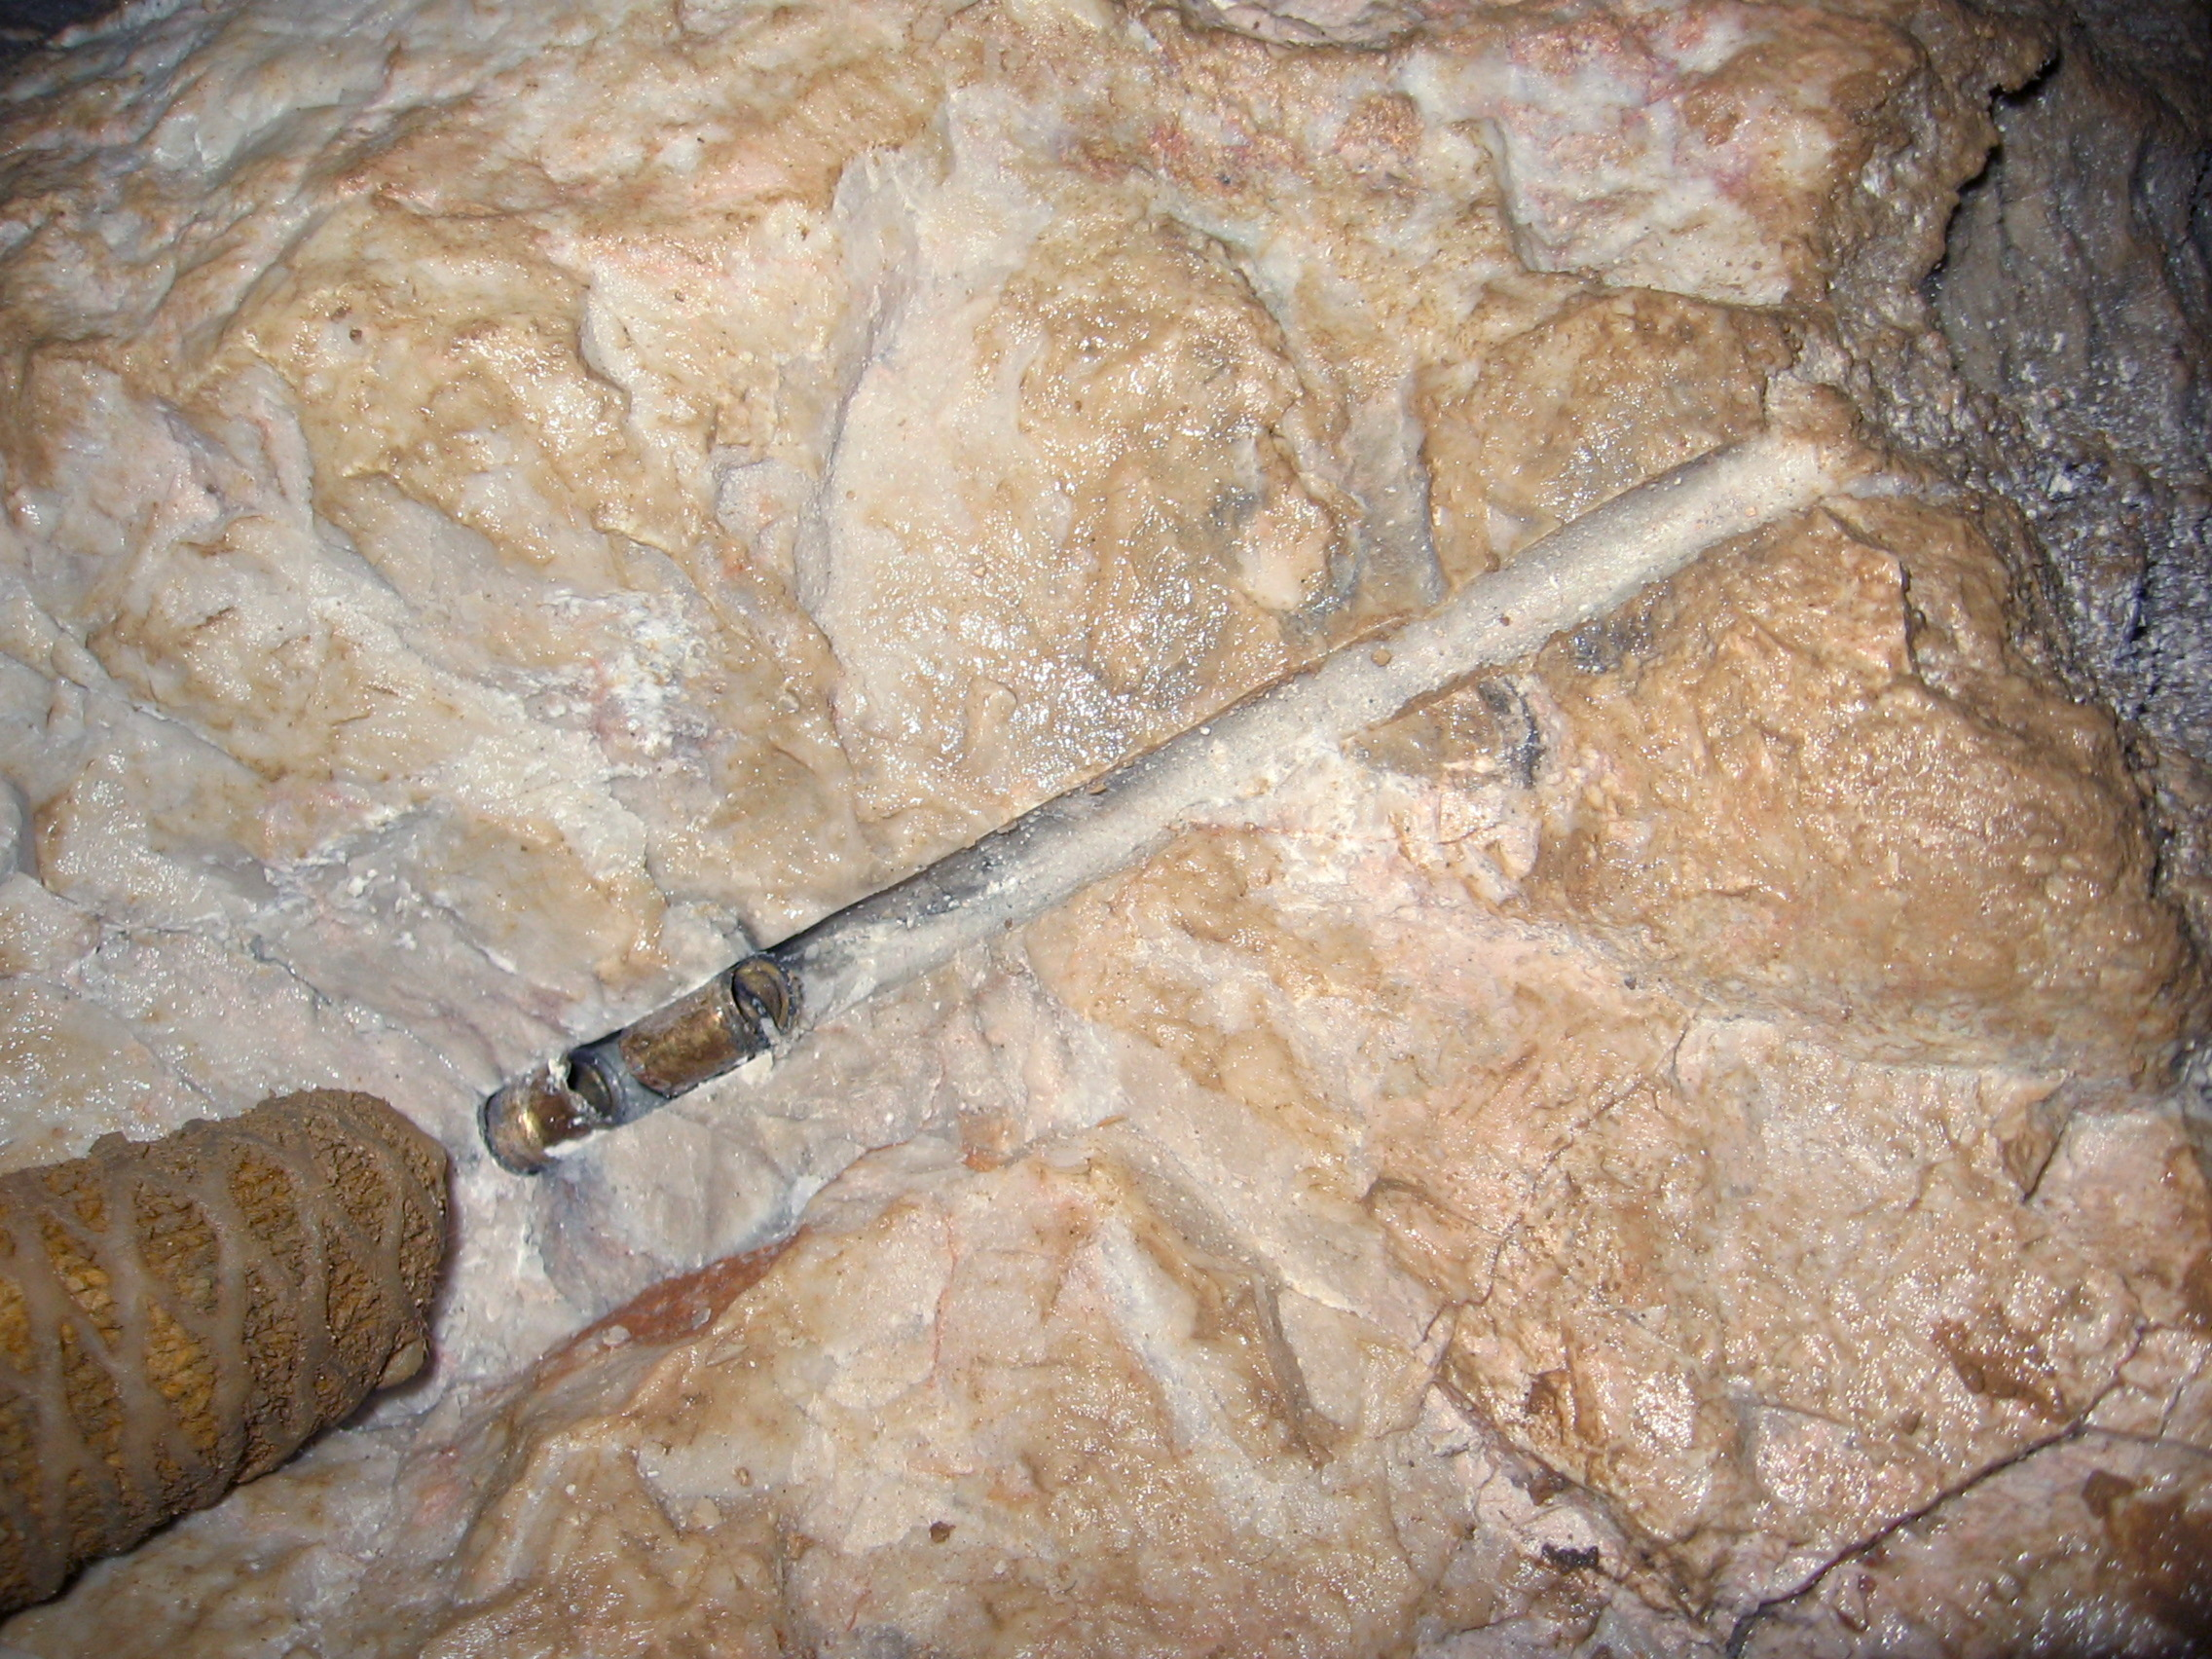
\includegraphics[width=\linewidth]{2009/e1logbook/opened pitch head--orig.jpg}}
        \caption{}
    \end{subfigure}
\hfill
    \begin{subfigure}{0.49\textwidth}
    \centering
        \frame{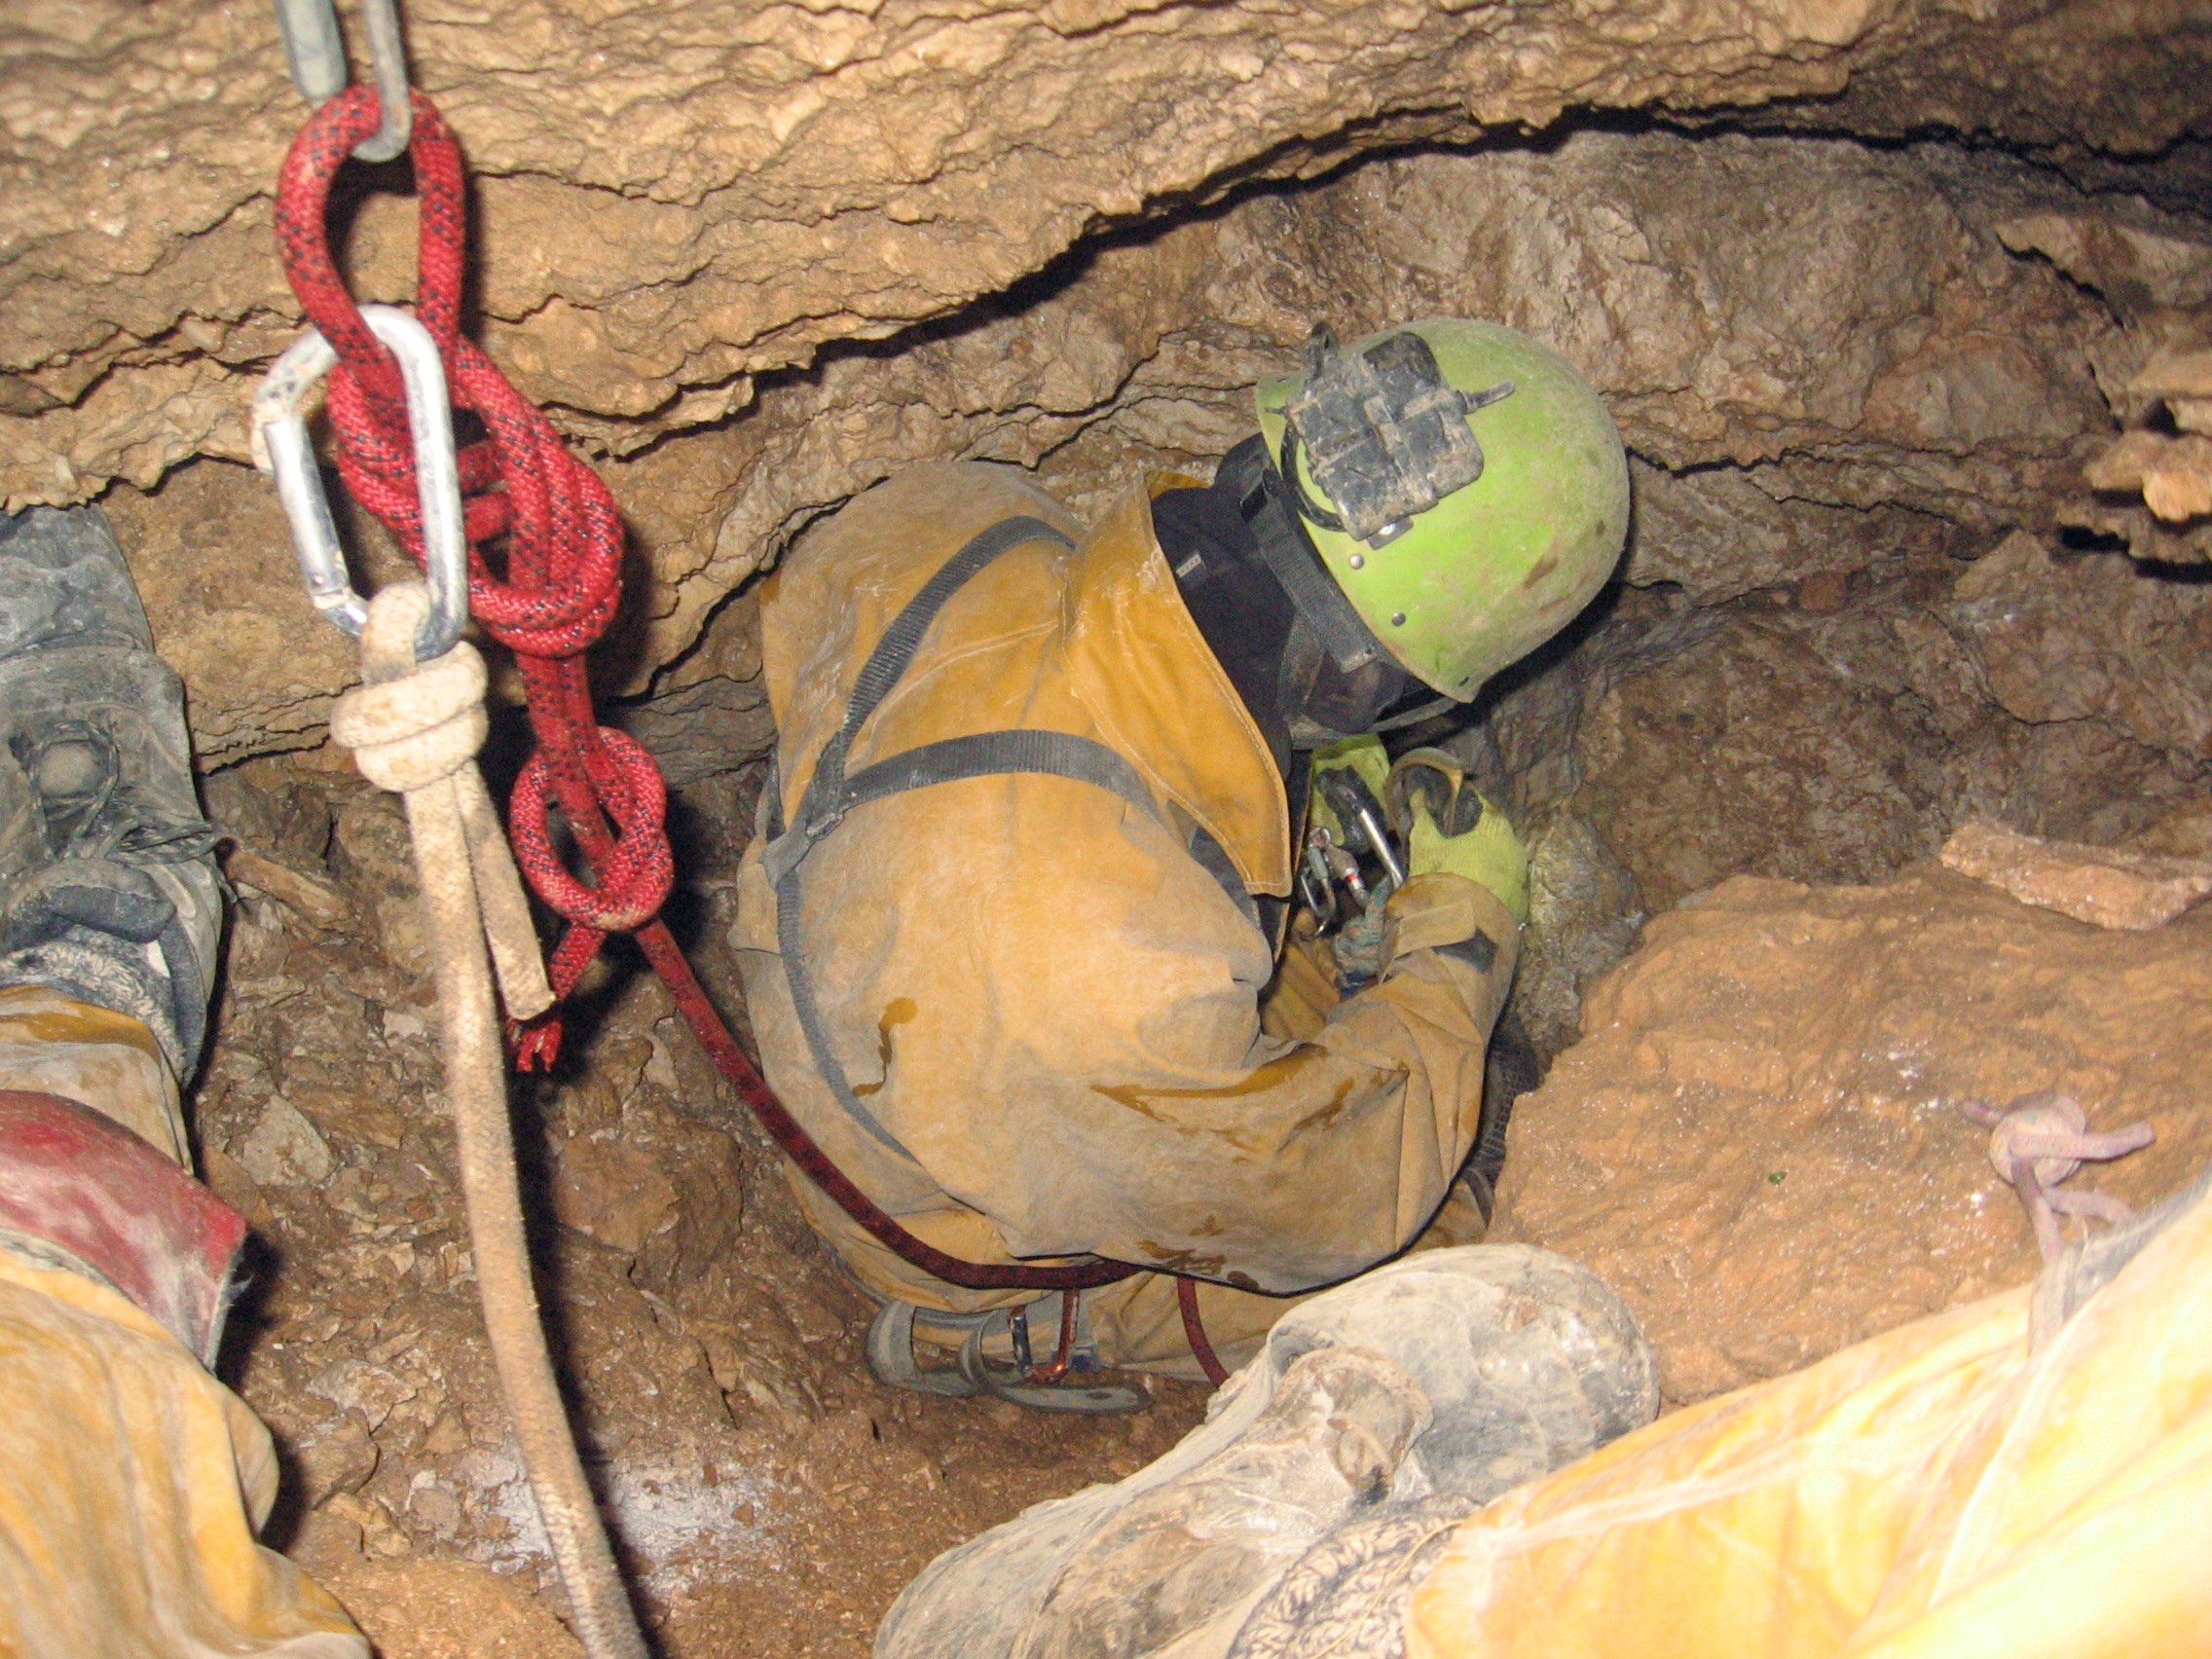
\includegraphics[width=\linewidth]{2009/e1logbook/preparing to descend the capped 2nd pitch for the first time--orig.jpg}}
        \caption{}
\end{subfigure}
\vfill
\begin{subfigure}{0.49\textwidth}
    \centering
        \frame{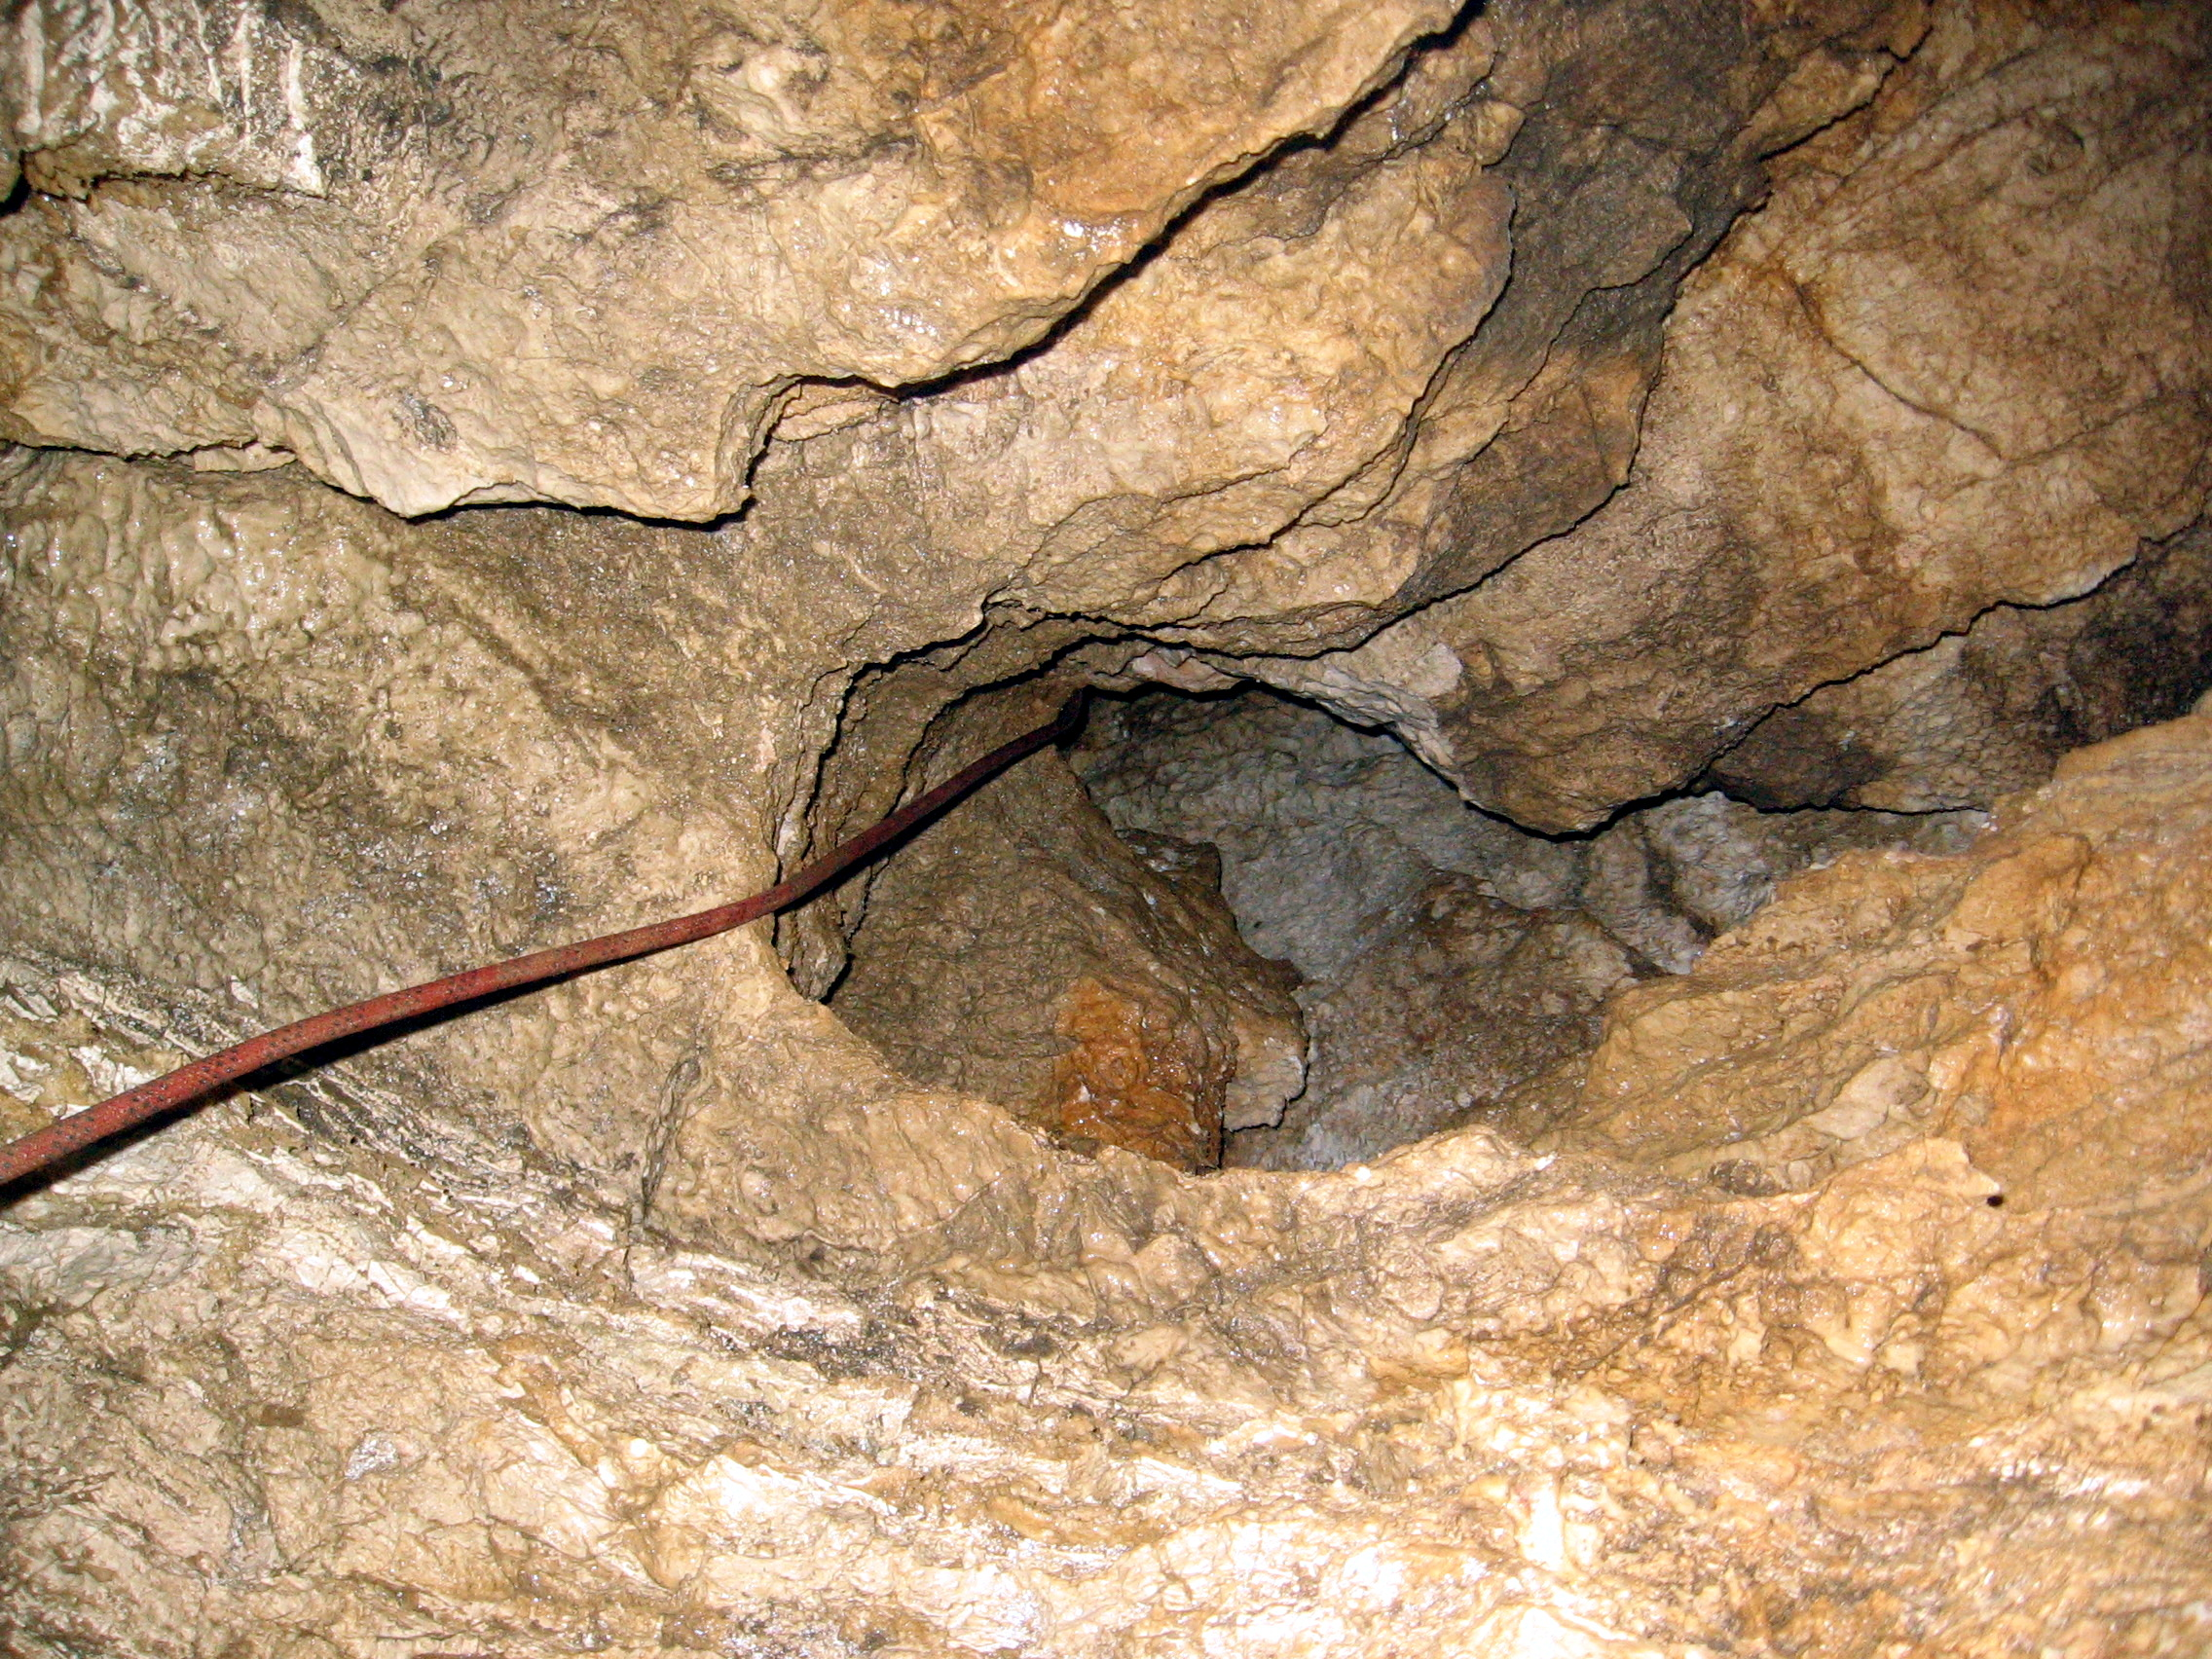
\includegraphics[width=\linewidth]{2009/e1logbook/looking back up 2nd pitch--orig.jpg}}
        \caption{}
\end{subfigure}
\hfill
\begin{subfigure}{0.49\textwidth}
    \centering
        \frame{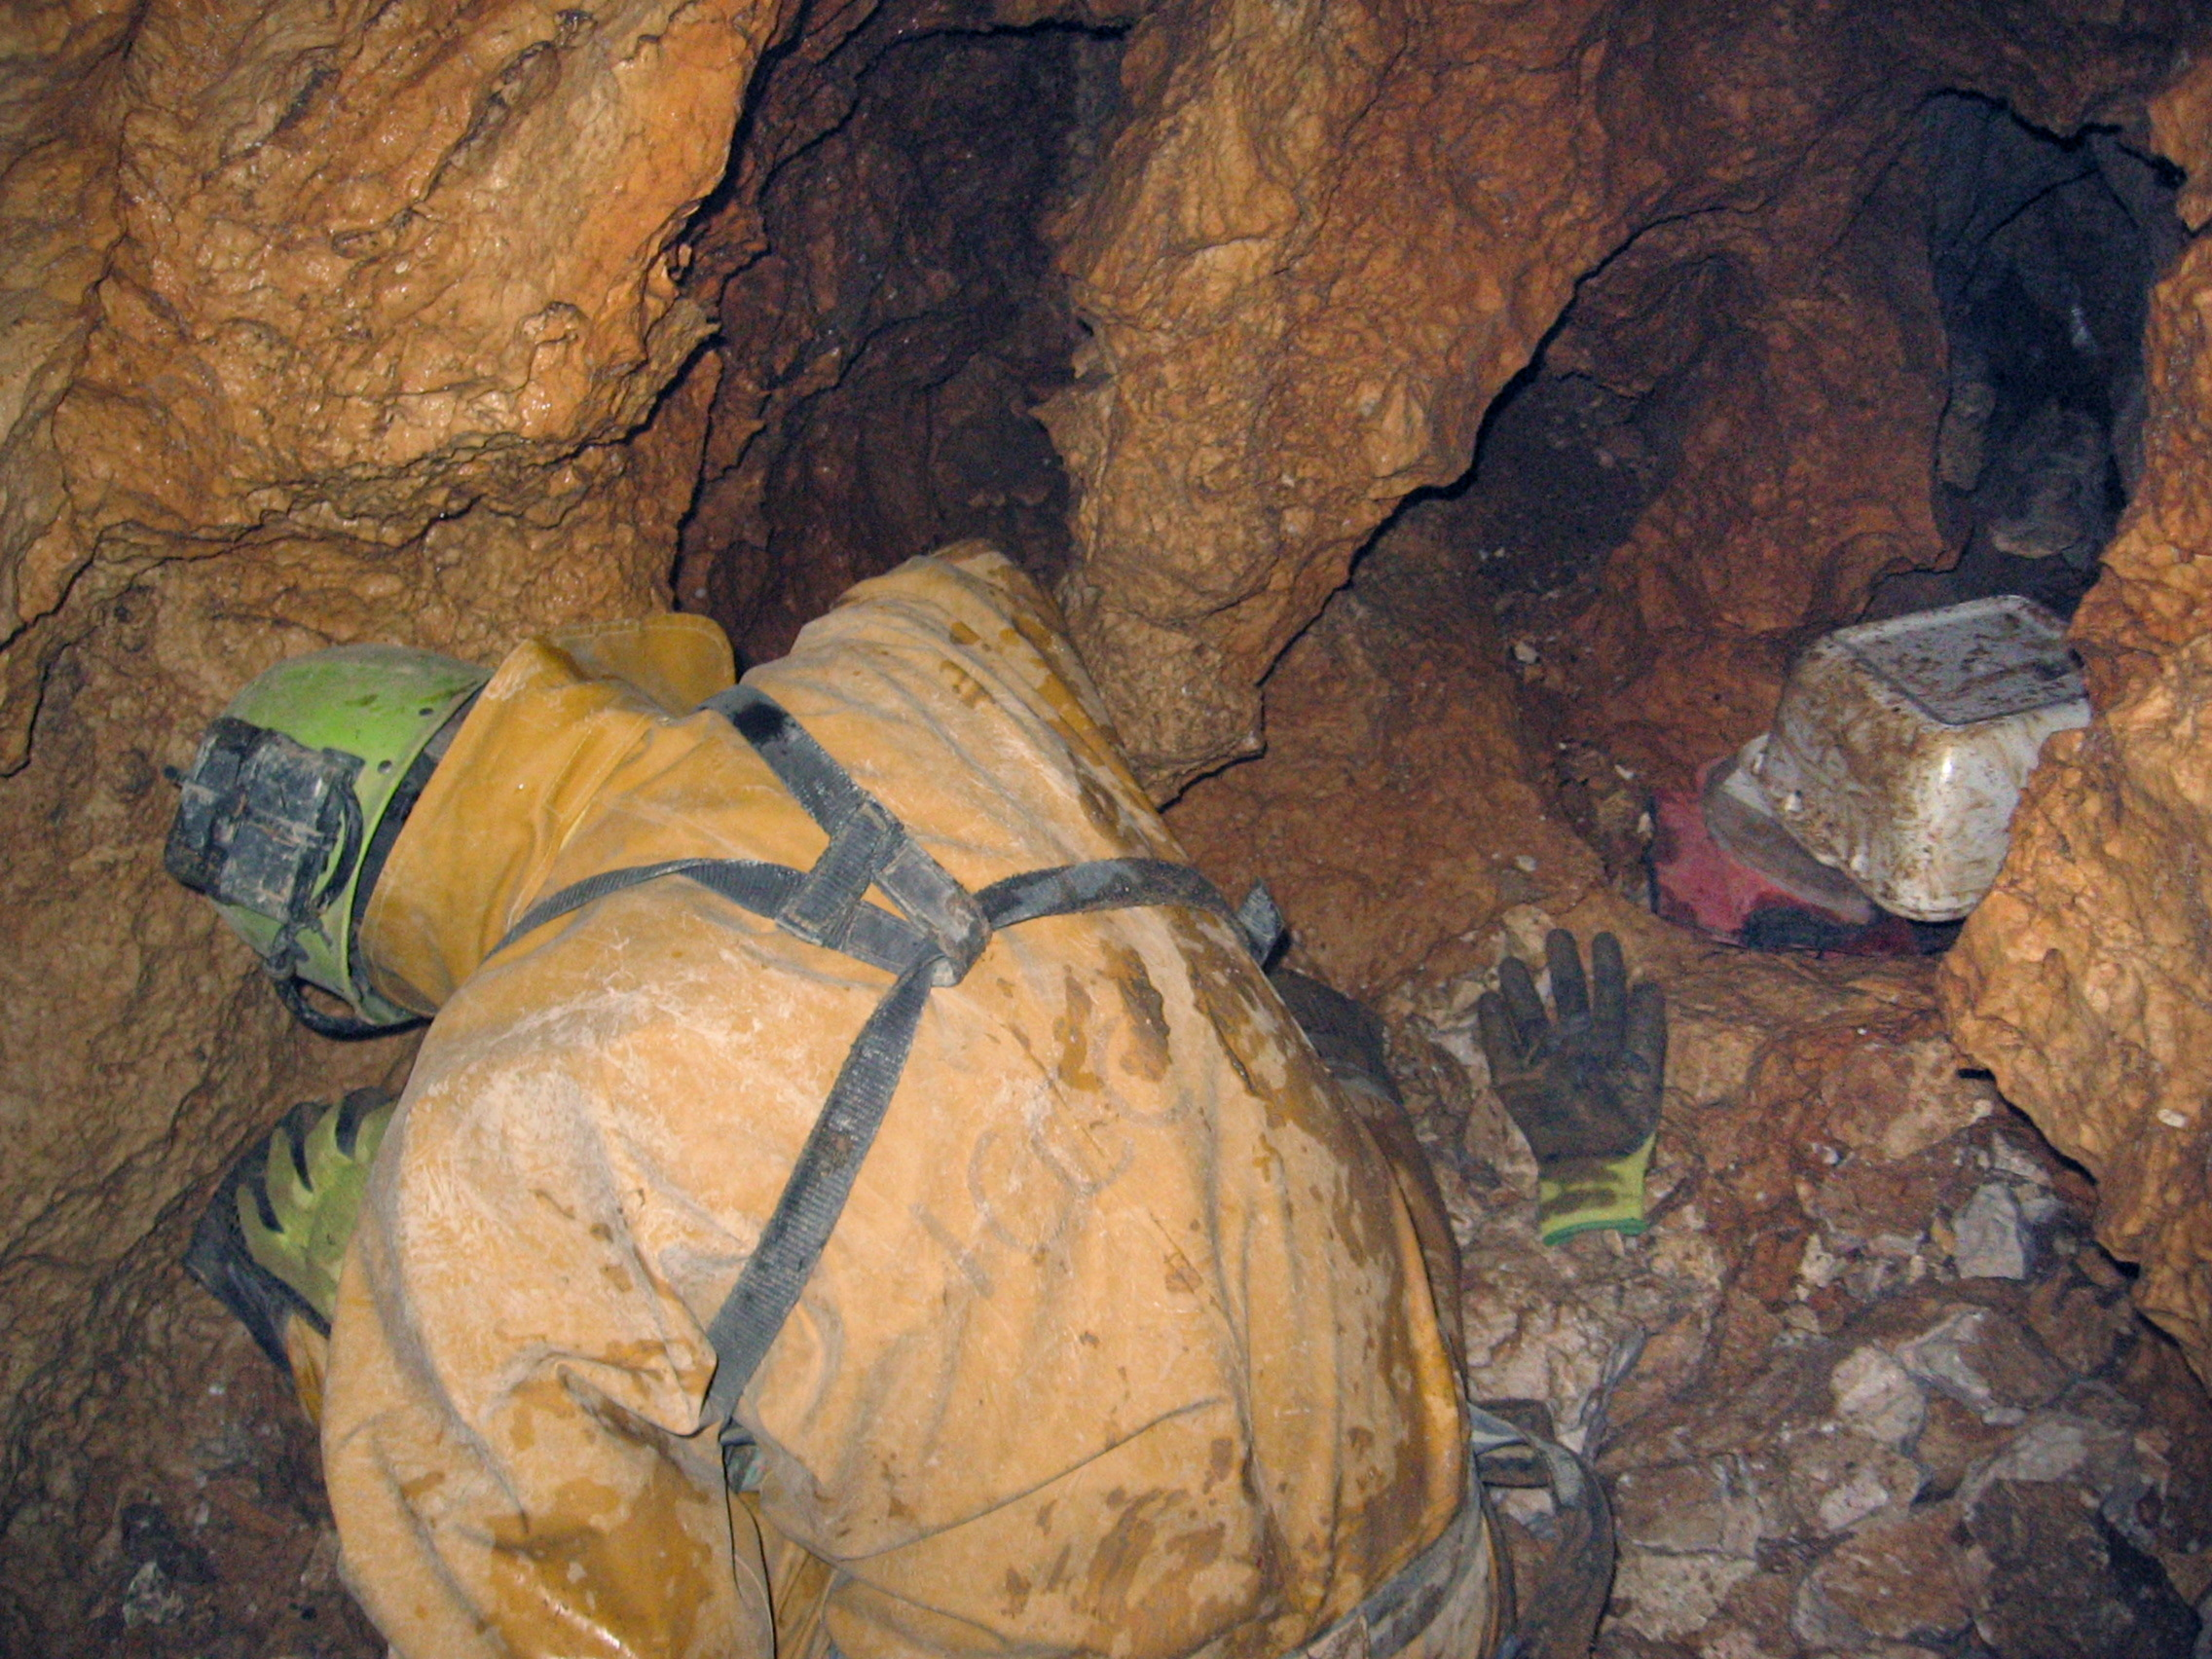
\includegraphics[width=\linewidth]{2009/e1logbook/Gergely digging at the new pushing front2--orig.jpg}}
        \caption{}
    \end{subfigure}
\vfill
\caption{Pushing the second pitch in \protect\passage{E1}. \textit{a)} The capped pitch head. \textit{b)} Gergely Ambrus preparing for the first descent of the second pitch. \textit{c)} Looking back up the pitch. \textit{d)} Gergely digging at the new pushing front. \pic{Jarvist Frost}}
\end{pagefigure}


